\documentclass[t, aspectratio=169]{beamer}
\usepackage{iftex}
\ifPDFTeX
	\usepackage[utf8]{inputenc}
	\usepackage[T5]{fontenc}
	\usepackage[vietnamese]{babel}
\else
	\usepackage{fontspec}
	\IfFontExistsTF{TeX Gyre Heros}{
		\setmainfont{TeX Gyre Heros}
		\setsansfont{TeX Gyre Heros}
	}{
		\setmainfont{Arial}[
			Path=/System/Library/Fonts/Supplemental/,
			Extension=.ttf,
			UprightFont=*,
			BoldFont=* Bold,
			ItalicFont=* Italic,
			BoldItalicFont=* Bold Italic
		]
		\setsansfont{Arial}[
			Path=/System/Library/Fonts/Supplemental/,
			Extension=.ttf,
			UprightFont=*,
			BoldFont=* Bold,
			ItalicFont=* Italic,
			BoldItalicFont=* Bold Italic
		]
	}
\fi
\usefonttheme{professionalfonts}
\usepackage{amsthm,amsmath,amssymb}
\usepackage{array}
\usepackage{tikz}
\usetikzlibrary{arrows.meta, positioning, shapes.geometric}

% --- CẤU HÌNH LỀ ---
\def\slideContentLeftMargin{0.5cm}
\def\slideContentRightMargin{1cm}
\def\hustHeaderHeight{1cm}
\def\slideContentBotMargin{3.5cm}

\usepackage[red, 169]{beamerthemeHUST}
\definecolor{hustprimary}{HTML}{ce1628}
\makeatletter
\renewcommand{\hust@colorname}{red}
\makeatother
\renewcommand{\hustbg}[1]{hust-red-169-#1.png}

\setbeamerfont{block title}{size=\normalsize,series=\bfseries}
\setbeamerfont{block body}{size=\small}
\setbeamerfont{itemize/enumerate body}{size=\small}
\setbeamerfont{itemize/enumerate subbody}{size=\scriptsize}
\setbeamercolor{structure}{fg=hustprimary}
\setbeamercolor{item}{fg=hustprimary}
\setbeamercolor{itemize item}{fg=hustprimary}
\setbeamercolor{itemize subitem}{fg=hustprimary}
\setbeamercolor{enumerate item}{fg=hustprimary}
\setbeamercolor{block title}{fg=hustprimary}
\setbeamercolor{block title alerted}{fg=hustprimary}
\setlength{\parskip}{0.12cm}

\renewcommand{\titlePageTitleX}{-0.5cm}
\renewcommand{\titlePageTitleY}{-0.5cm}
\renewcommand{\hustTitleAlign}{\alignLeft}
\renewcommand{\hustSubtitleAlign}{\alignLeft}
\renewcommand{\hustAuthorAlign}{\alignLeft}
\renewcommand{\hustInstAlign}{\alignLeft}

\title{BKADVISOR: CHATBOT TƯ VẤN SINH VIÊN}
\subtitle{RAG học vụ có truy hồi lai, định tuyến theo độ phức tạp và kiểm soát nguồn}
\author{\texorpdfstring{Nguyễn Hoài Nam \\ GVHD: TS. Cao Tuấn Dũng}{Nguyễn Hoài Nam, GVHD: TS. Cao Tuấn Dũng}}
\institute{Chương trình Công nghệ thông tin Việt--Nhật}

\newcommand{\agendaColor}{%
	\ifnum\value{section}=0
		\color{black}\bfseries
	\else
		\color{black!28}\bfseries
	\fi
}

\setbeamertemplate{section in toc}{%
	\leavevmode
	\leftskip=1.5em
	\ifnum\inserttocsectionnumber=\value{section}
		{\color{black}\bfseries\Large\inserttocsectionnumber.\hskip1.25em\inserttocsection}
	\else
		{\agendaColor\Large\inserttocsectionnumber.\hskip1.25em\inserttocsection}
	\fi
	\par\vspace{0.35cm}
}

\newcommand{\agendaItem}[2]{%
	\par\noindent
	\ifnum\value{section}=#1
		{\color{black}\bfseries\Large #1. #2}
	\else
		\ifnum\value{section}=0
			{\color{black}\bfseries\Large #1. #2}
		\else
			{\color{black!28}\bfseries\Large #1. #2}
		\fi
	\fi
	\par\vspace{0.34cm}
}

\newcommand{\agendaFrame}{
	{
		\setbeamertemplate{background}{
			\begin{tikzpicture}[remember picture, overlay]
				\node[anchor=south west, inner sep=0pt] at (current page.south west)
				{
\includegraphics[width=\paperwidth,height=\paperheight]{hust-red-169-content-hust-full.png}};
				\begin{scope}
					\clip (current page.south west) rectangle ([xshift=0.37\paperwidth]current page.north west);
					\node[anchor=south west, inner sep=0pt]
					at (current page.south west)
					{
\includegraphics[height=\paperheight]{hust-red-169-section.png}};
				\end{scope}
				\fill[white] ([xshift=0.37\paperwidth]current page.south west) rectangle (current page.north east);
				\node[
					font=\bfseries\fontsize{34}{38}\selectfont,
					text=white
				] at ([xshift=-0.31\paperwidth]current page.center) {HUST};
				\node[
					anchor=south west,
					font=\scriptsize\bfseries,
					text=white
				] at ([xshift=0.035\paperwidth,yshift=0.45cm]current page.south west)
				{hust.edu.vn \quad fb.com/dhbkhn};
			\end{tikzpicture}
			\drawHustPageNum
		}
		\begin{frame}[plain]
			\begin{tikzpicture}[remember picture, overlay]
				\node[anchor=north west, inner sep=0pt]
				at ([xshift=0.39\paperwidth,yshift=-0.65cm]current page.north west)
				{
					\begin{minipage}{0.59\paperwidth}
						\centering
						{\color{hustprimary}\bfseries\fontsize{24}{28}\selectfont NỘI DUNG TRÌNH BÀY\par}
						\vspace{0.45cm}
						\raggedright
						\agendaItem{1}{Đặt vấn đề}
						\agendaItem{2}{Phân tích yêu cầu}
						\agendaItem{3}{Công nghệ sử dụng}
						\agendaItem{4}{Thiết kế và xây dựng hệ thống}
						\agendaItem{5}{Đóng góp nổi bật}
						\agendaItem{6}{Kết luận và hướng phát triển}
					\end{minipage}
				};
			\end{tikzpicture}
		\end{frame}
	}
}

\newif\ifShowSectionAgenda
\ShowSectionAgendafalse
\AtBeginSection[]{
	\ifShowSectionAgenda
		\agendaFrame
	\else
		\global\ShowSectionAgendatrue
	\fi
}

\begin{document}

	\husttitlepage

	\resetPageCount
	\showPageNumber
	\useStyleHustFull
	\useThinBar
	\agendaFrame

	% ================================================================
	\section{Đặt vấn đề}

	\begin{frame}{Ba vấn đề chính}
		\begin{columns}[T,onlytextwidth]
			\begin{column}{0.32\textwidth}
				\begin{block}{Thông tin phân tán}
					CTĐT, quy định, kế hoạch, thông báo và thủ tục nằm ở nhiều nguồn khác nhau.
				\end{block}
			\end{column}
			\begin{column}{0.32\textwidth}
				\begin{block}{Câu hỏi tự nhiên}
					Sinh viên hỏi bằng tiếng Việt đời thường, có mã học phần, khóa, ngành hoặc ngữ cảnh.
				\end{block}
			\end{column}
			\begin{column}{0.32\textwidth}
				\begin{block}{Cần căn cứ rõ ràng}
					Câu trả lời sai nguồn hoặc lỗi thời có thể dẫn đến quyết định học vụ sai.
				\end{block}
			\end{column}
		\end{columns}

		\vspace{0.6cm}
		\centering
		\textbf{Bài toán:} xây dựng trợ lý học vụ hỏi đáp tự nhiên, truy hồi đúng nguồn và trả lời có thể kiểm chứng.
	\end{frame}

	\begin{frame}{Mục tiêu của BKAdvisor}
		\begin{columns}[T,onlytextwidth]
			\begin{column}{0.48\textwidth}
				\begin{block}{Trải nghiệm hỏi đáp}
					\begin{itemize}
						\item Nhận câu hỏi tiếng Việt tự nhiên.
						\item Trả lời dựa trên tài liệu đã truy hồi.
						\item Hiển thị nguồn và metadata để kiểm chứng.
					\end{itemize}
				\end{block}
			\end{column}
			\begin{column}{0.48\textwidth}
				\begin{block}{Vận hành tri thức}
					\begin{itemize}
						\item Tổ chức kho tri thức theo miền học vụ.
						\item Hỗ trợ upload, review và index tài liệu mới.
						\item Theo dõi trace, feedback và metric chất lượng.
					\end{itemize}
				\end{block}
			\end{column}
		\end{columns}
	\end{frame}

	% ================================================================
	\section{Phân tích yêu cầu}

	\begin{frame}{Use case trọng tâm}
		\begin{columns}[T,onlytextwidth]
			\begin{column}{0.48\textwidth}
				\begin{block}{UC01 -- Sinh viên chat học vụ}
					\begin{itemize}
						\item Sinh viên gửi câu hỏi tiếng Việt tự nhiên.
						\item Hệ thống truy hồi tài liệu học vụ phù hợp.
						\item Trả lời trong phiên hội thoại, kèm nguồn và metadata để kiểm chứng.
					\end{itemize}
				\end{block}
			\end{column}
			\begin{column}{0.48\textwidth}
				\begin{block}{UC02 -- Admin upload và index tài liệu}
					\begin{itemize}
						\item Admin tải PDF/DOCX hoặc duyệt dữ liệu crawler.
						\item Hệ thống chuyển đổi, chuẩn hóa, chunk và tạo embedding.
						\item Admin review trước khi index vào Qdrant và Elasticsearch.
					\end{itemize}
				\end{block}
			\end{column}
		\end{columns}

		\vspace{0.25cm}
		\begin{alertblock}{Phân định phạm vi}
			\small Các thao tác như xem nguồn, metadata, session, bookmark hay feedback là chức năng trong luồng UC01, không tách thành use case trọng tâm.
		\end{alertblock}
	\end{frame}

	\begin{frame}{Phạm vi dữ liệu và chức năng}
		\begin{columns}[T,onlytextwidth]
			\begin{column}{0.48\textwidth}
				\begin{block}{Bốn collection}
					\begin{itemize}
						\item \texttt{ctdt}: CTĐT, học phần, tín chỉ, tiên quyết.
						\item \texttt{quydinh}: quy chế, học bổng, tốt nghiệp.
						\item \texttt{kehoach}: kế hoạch học kỳ, thông báo, deadline.
						\item \texttt{stsv}: thủ tục, biểu mẫu, hỗ trợ sinh viên.
					\end{itemize}
				\end{block}
			\end{column}
			\begin{column}{0.48\textwidth}
				\begin{block}{Nhóm chức năng}
					\begin{itemize}
						\item Chat thường, metadata và streaming.
						\item Session, auth, bookmark, feedback.
						\item Upload, review và index tài liệu.
						\item Evaluation, trace và notification.
					\end{itemize}
				\end{block}
			\end{column}
		\end{columns}
	\end{frame}

	% ================================================================
	\section{Công nghệ sử dụng}

	\begin{frame}{Công nghệ theo vai trò}
		\small
		\centering
		\begin{minipage}{0.92\textwidth}
			\scriptsize\textbf{Nguyên tắc chọn:} ưu tiên công nghệ phục vụ nhập dữ liệu, truy hồi, kiểm soát nguồn và vận hành RAG học vụ.
		\end{minipage}
		\vspace{0.08cm}

		\begin{columns}[T,onlytextwidth]
			\begin{column}{0.48\textwidth}
				\begin{block}{Giao diện}
					\begin{itemize}
						\item React/Vite cho web app.
						\item Expo/React Native cho mobile app.
						\item TypeScript package dùng chung API contract.
					\end{itemize}
				\end{block}
				\begin{block}{Backend}
					\begin{itemize}
						\item FastAPI điều phối chat, streaming, session.
						\item Auth, document admin, feedback, lookup, notification.
					\end{itemize}
				\end{block}
			\end{column}
			\begin{column}{0.48\textwidth}
				\begin{block}{Dữ liệu}
					\begin{itemize}
						\item MongoDB lưu nghiệp vụ.
						\item Redis cache, session, rate limit.
						\item Qdrant vector; Elasticsearch BM25.
					\end{itemize}
				\end{block}
				\begin{block}{AI/Search}
					\begin{itemize}
						\item BGE-M3, E5 multilingual, BGE reranker.
						\item LangGraph agent, LLM generation.
					\end{itemize}
				\end{block}
			\end{column}
		\end{columns}
	\end{frame}

	% ================================================================
	\section{Thiết kế và xây dựng hệ thống}

	\begin{frame}{Kiến trúc tổng thể}
		\centering
		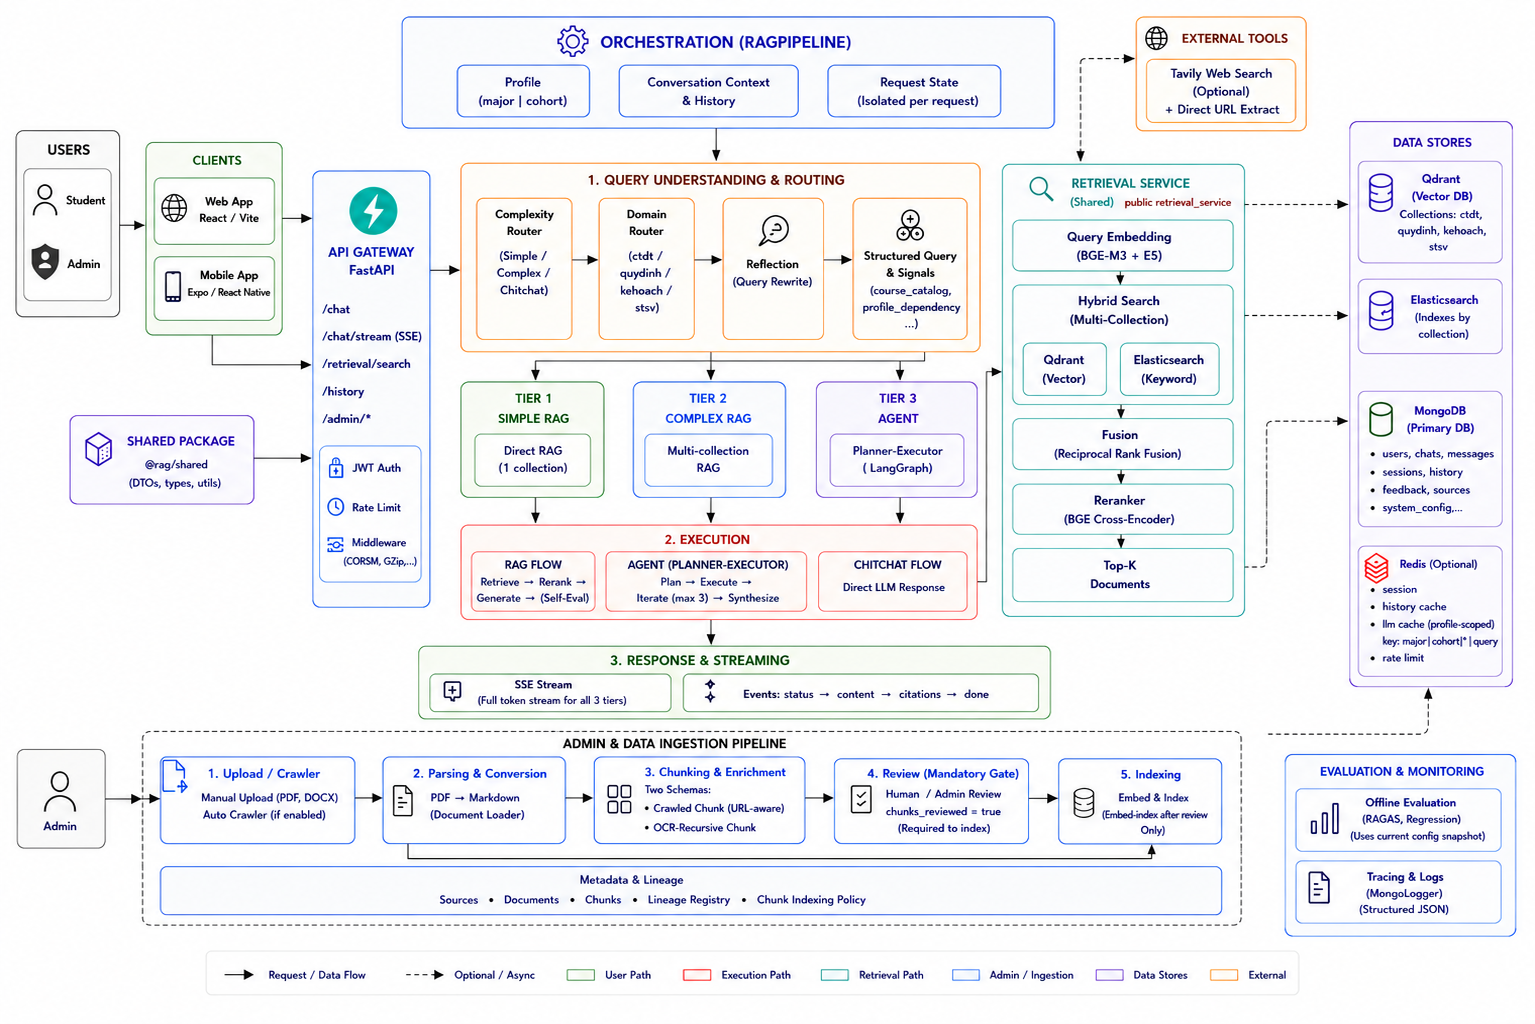
\includegraphics[width=0.96\textwidth,height=5.7cm,keepaspectratio]{figures/system_design.png}

		\vspace{0.1cm}
		\scriptsize
		\textbf{Luồng chính:} Client $\rightarrow$ FastAPI $\rightarrow$ RAGPipeline/DocumentPipeline $\rightarrow$ Retrieval service $\rightarrow$ MongoDB/Qdrant/Elasticsearch/Redis.
	\end{frame}

	\begin{frame}{Thiết kế dữ liệu}
		\begin{columns}[T,onlytextwidth]
			\begin{column}{0.48\textwidth}
				\begin{block}{MongoDB}
					\begin{itemize}
						\item \texttt{users}, \texttt{sessions}, \texttt{chat\_turns}.
						\item \texttt{documents}, \texttt{chunks}, \texttt{agent\_traces}.
						\item \texttt{bookmarks}, \texttt{feedback}, \texttt{notifications}.
					\end{itemize}
				\end{block}
			\end{column}
			\begin{column}{0.48\textwidth}
				\begin{block}{Kho truy hồi}
					\begin{itemize}
						\item Qdrant lưu vector BGE-M3 và E5 theo collection.
						\item Elasticsearch lưu BM25 với Vietnamese analyzer + \texttt{vi\_tokenizer}.
						\item Redis cache session, history, response và rate limit.
					\end{itemize}
				\end{block}
			\end{column}
		\end{columns}

		\vspace{0.3cm}
		\centering
		\small\textbf{Định danh tham chiếu liên kho:} \texttt{document\_id}, \texttt{chunk\_id}, collection, source/version và trạng thái hiệu lực.
	\end{frame}

	\begin{frame}{Luồng hỏi đáp RAGPipeline}
		\begin{columns}[T,onlytextwidth]
			\begin{column}{0.32\textwidth}
				\begin{block}{1. Hiểu truy vấn}
					\begin{itemize}
						\item Viết lại câu hỏi khi cần.
						\item Nhận diện miền và thực thể học vụ.
						\item Chọn chitchat, Simple RAG hoặc Agent.
					\end{itemize}
				\end{block}
			\end{column}
			\begin{column}{0.32\textwidth}
				\begin{block}{2. Truy hồi}
					\begin{itemize}
						\item Vector search trên Qdrant.
						\item BM25 trên Elasticsearch.
						\item Rerank và lọc hiệu lực tài liệu.
					\end{itemize}
				\end{block}
			\end{column}
			\begin{column}{0.32\textwidth}
				\begin{block}{3. Trả lời}
					\begin{itemize}
						\item Bổ sung tham chiếu điều khoản.
						\item Sinh câu trả lời có nguồn.
						\item Lưu trace, feedback và metadata.
					\end{itemize}
				\end{block}
			\end{column}
		\end{columns}
	\end{frame}

	\begin{frame}{Luồng xử lý dữ liệu}
		\begin{columns}[T,onlytextwidth]
			\begin{column}{0.48\textwidth}
				\begin{block}{Đầu vào}
					\begin{itemize}
						\item Tài liệu PDF/DOCX do admin upload.
						\item Nội dung web do crawler thu thập.
						\item Metadata nguồn, miền dữ liệu và trạng thái xử lý.
					\end{itemize}
				\end{block}
			\end{column}
			\begin{column}{0.48\textwidth}
				\begin{block}{Các bước chính}
					\begin{enumerate}
						\item Convert sang Markdown.
						\item LLM chuẩn hóa Markdown: heading, bảng, danh sách.
						\item Làm sạch và chunk theo miền.
						\item Admin review.
						\item Embedding BGE-M3/E5.
						\item Index vào Qdrant và Elasticsearch.
					\end{enumerate}
				\end{block}
			\end{column}
		\end{columns}

		\vspace{0.25cm}
		\centering
		\small\textbf{Human gate:} admin review trước khi index để ngăn chunk lỗi, metadata sai hoặc bảng/heading bị méo đi vào kho tri thức.
	\end{frame}

	\begin{frame}{Minh họa sản phẩm: hỏi đáp sinh viên}
		\begin{columns}[T,onlytextwidth]
			\begin{column}{0.34\textwidth}
				\begin{block}{Màn hình chào}
					\small Gợi ý câu hỏi theo chủ đề học vụ, thanh nhập câu hỏi và lịch sử phiên hội thoại.
				\end{block}
				\begin{block}{Câu trả lời}
					\small Nội dung trả lời có cấu trúc, trích dẫn nguồn, metadata và trạng thái xử lý.
				\end{block}
				\begin{block}{Tương tác}
					\small Streaming, bookmark, feedback và tiếp tục hỏi trong cùng ngữ cảnh hội thoại.
				\end{block}
			\end{column}
			\begin{column}{0.62\textwidth}
				\centering
				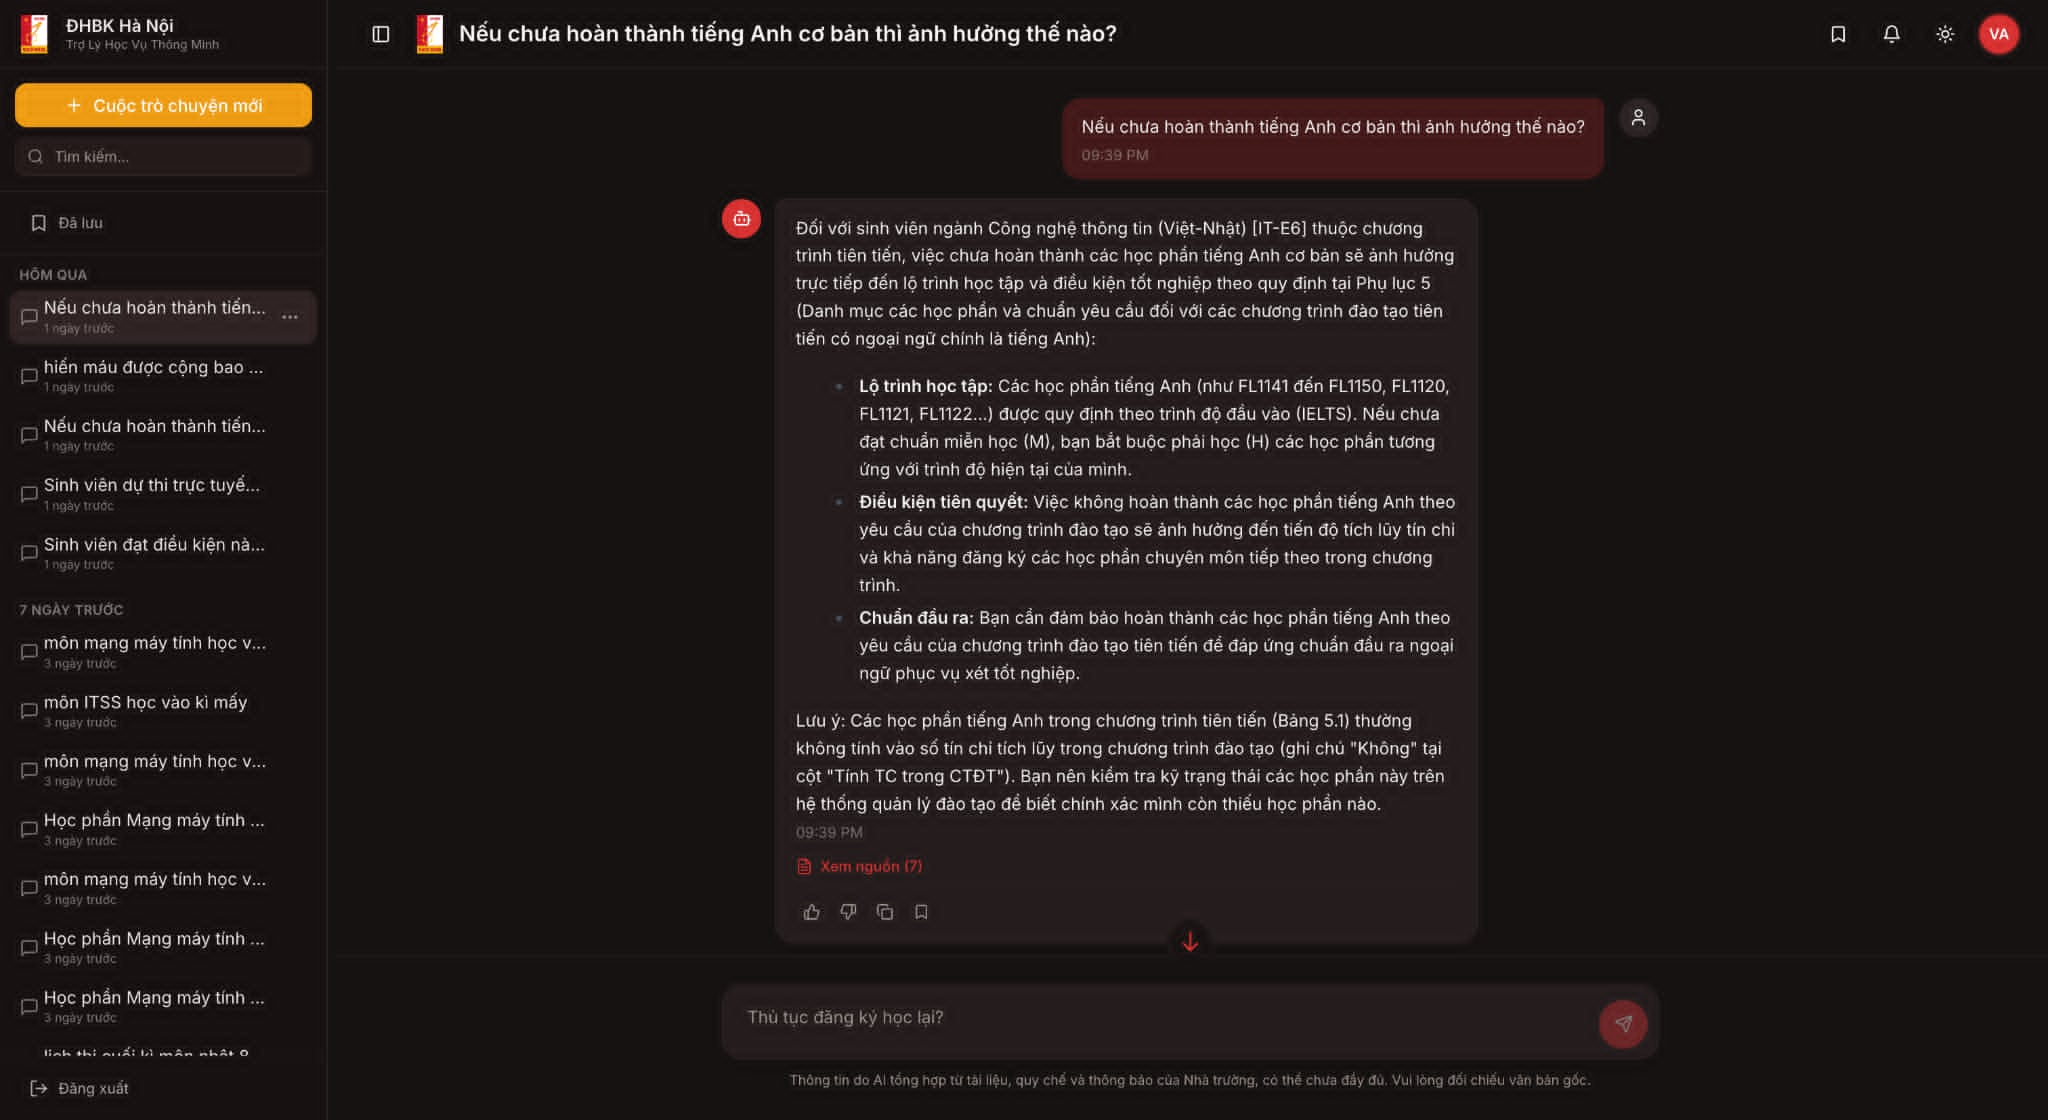
\includegraphics[width=\textwidth,height=5.45cm,keepaspectratio]{figures/ui_chat_long.jpg}
			\end{column}
		\end{columns}
	\end{frame}

	\begin{frame}{Minh họa sản phẩm: quản trị tri thức}
		\begin{columns}[T,onlytextwidth]
			\begin{column}{0.34\textwidth}
				\begin{block}{Upload}
					\small Admin tải PDF/DOCX, chọn collection, thêm metadata nguồn và theo dõi trạng thái xử lý.
				\end{block}
				\begin{block}{Review}
					\small Kiểm tra chunk, nội dung Markdown, metadata và lỗi chuyển đổi trước khi index.
				\end{block}
				\begin{block}{Index/Evaluate}
					\small Đưa dữ liệu vào Qdrant, Elasticsearch và chạy đánh giá hồi quy sau khi cập nhật.
				\end{block}
			\end{column}
			\begin{column}{0.62\textwidth}
				\centering
				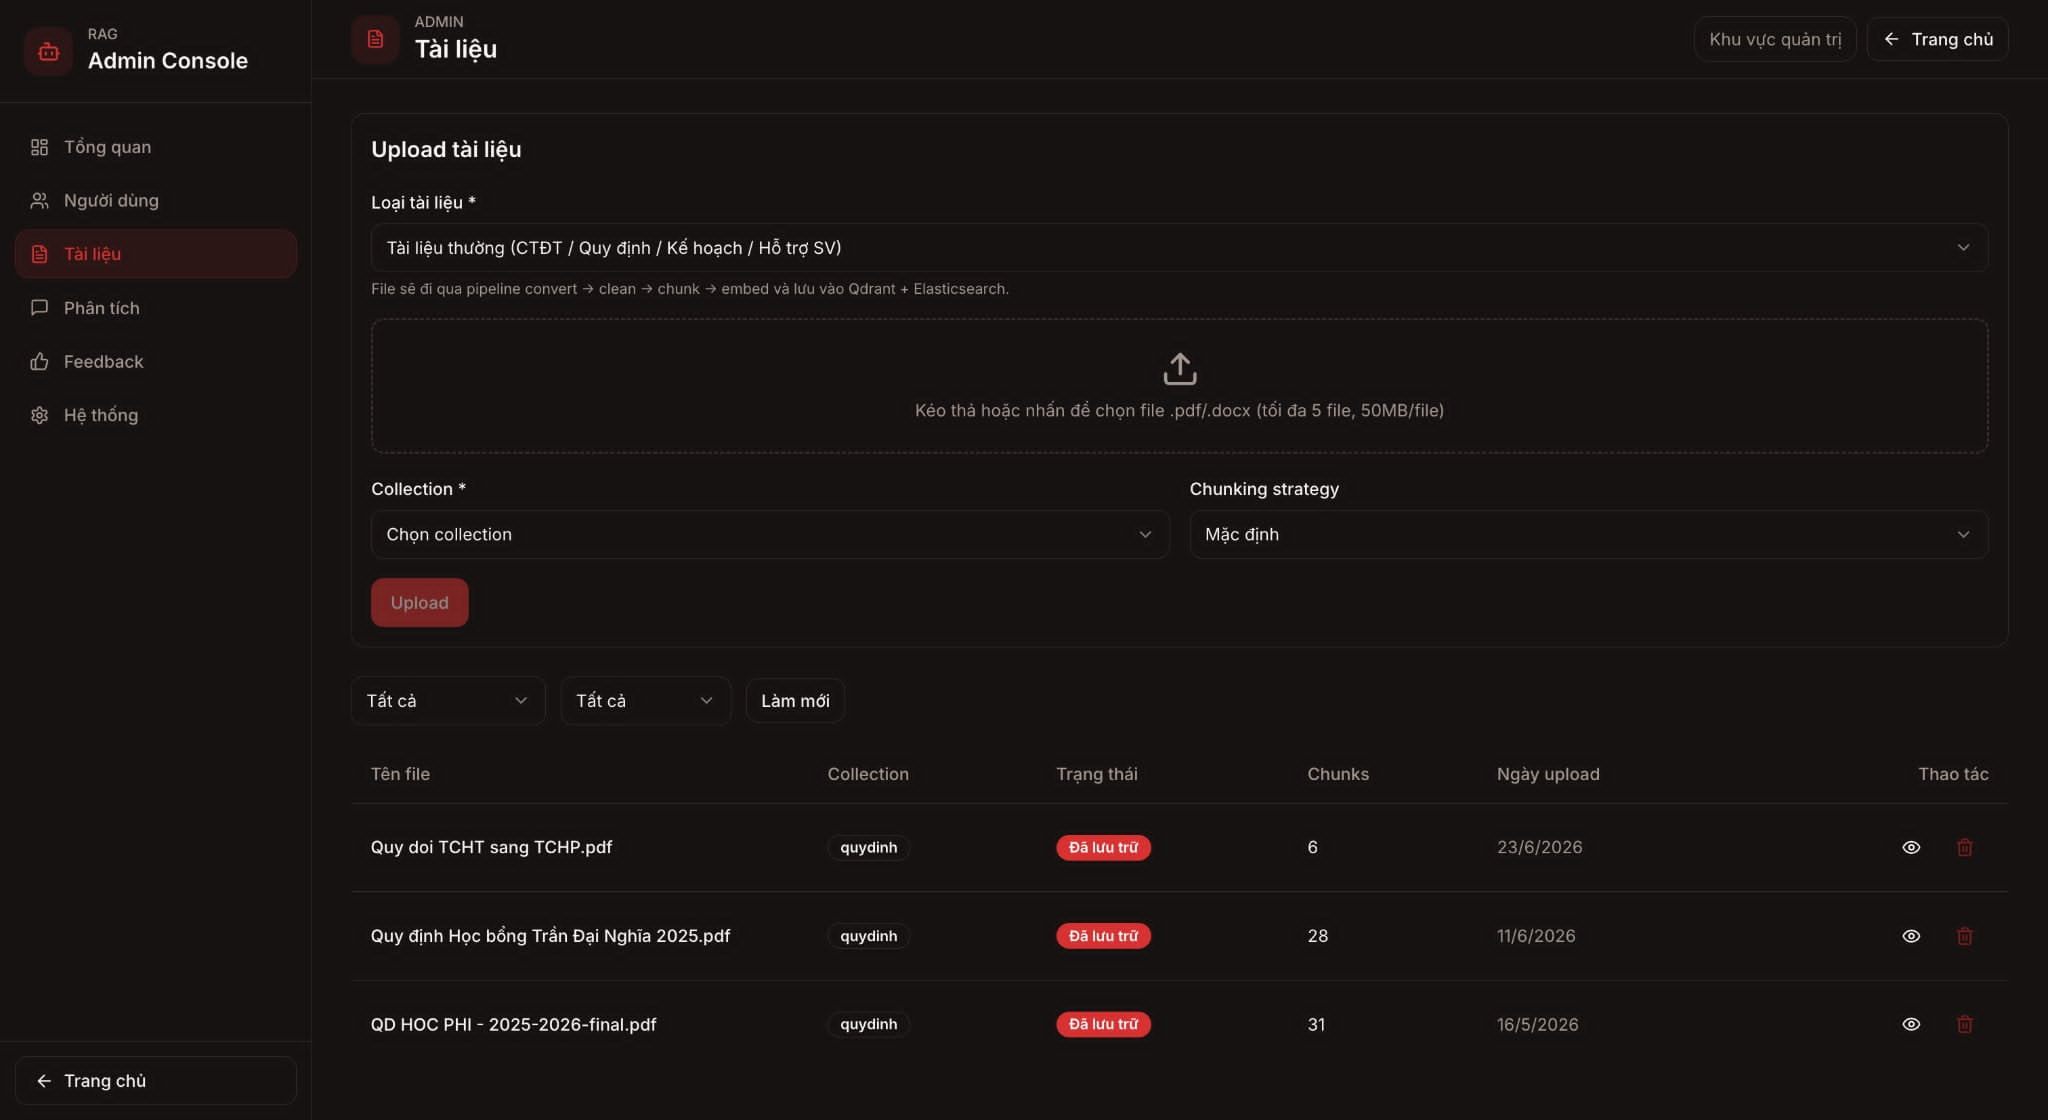
\includegraphics[width=\textwidth,height=2.62cm,keepaspectratio]{figures/ui_admin_upload.jpg}
				\vspace{0.08cm}

				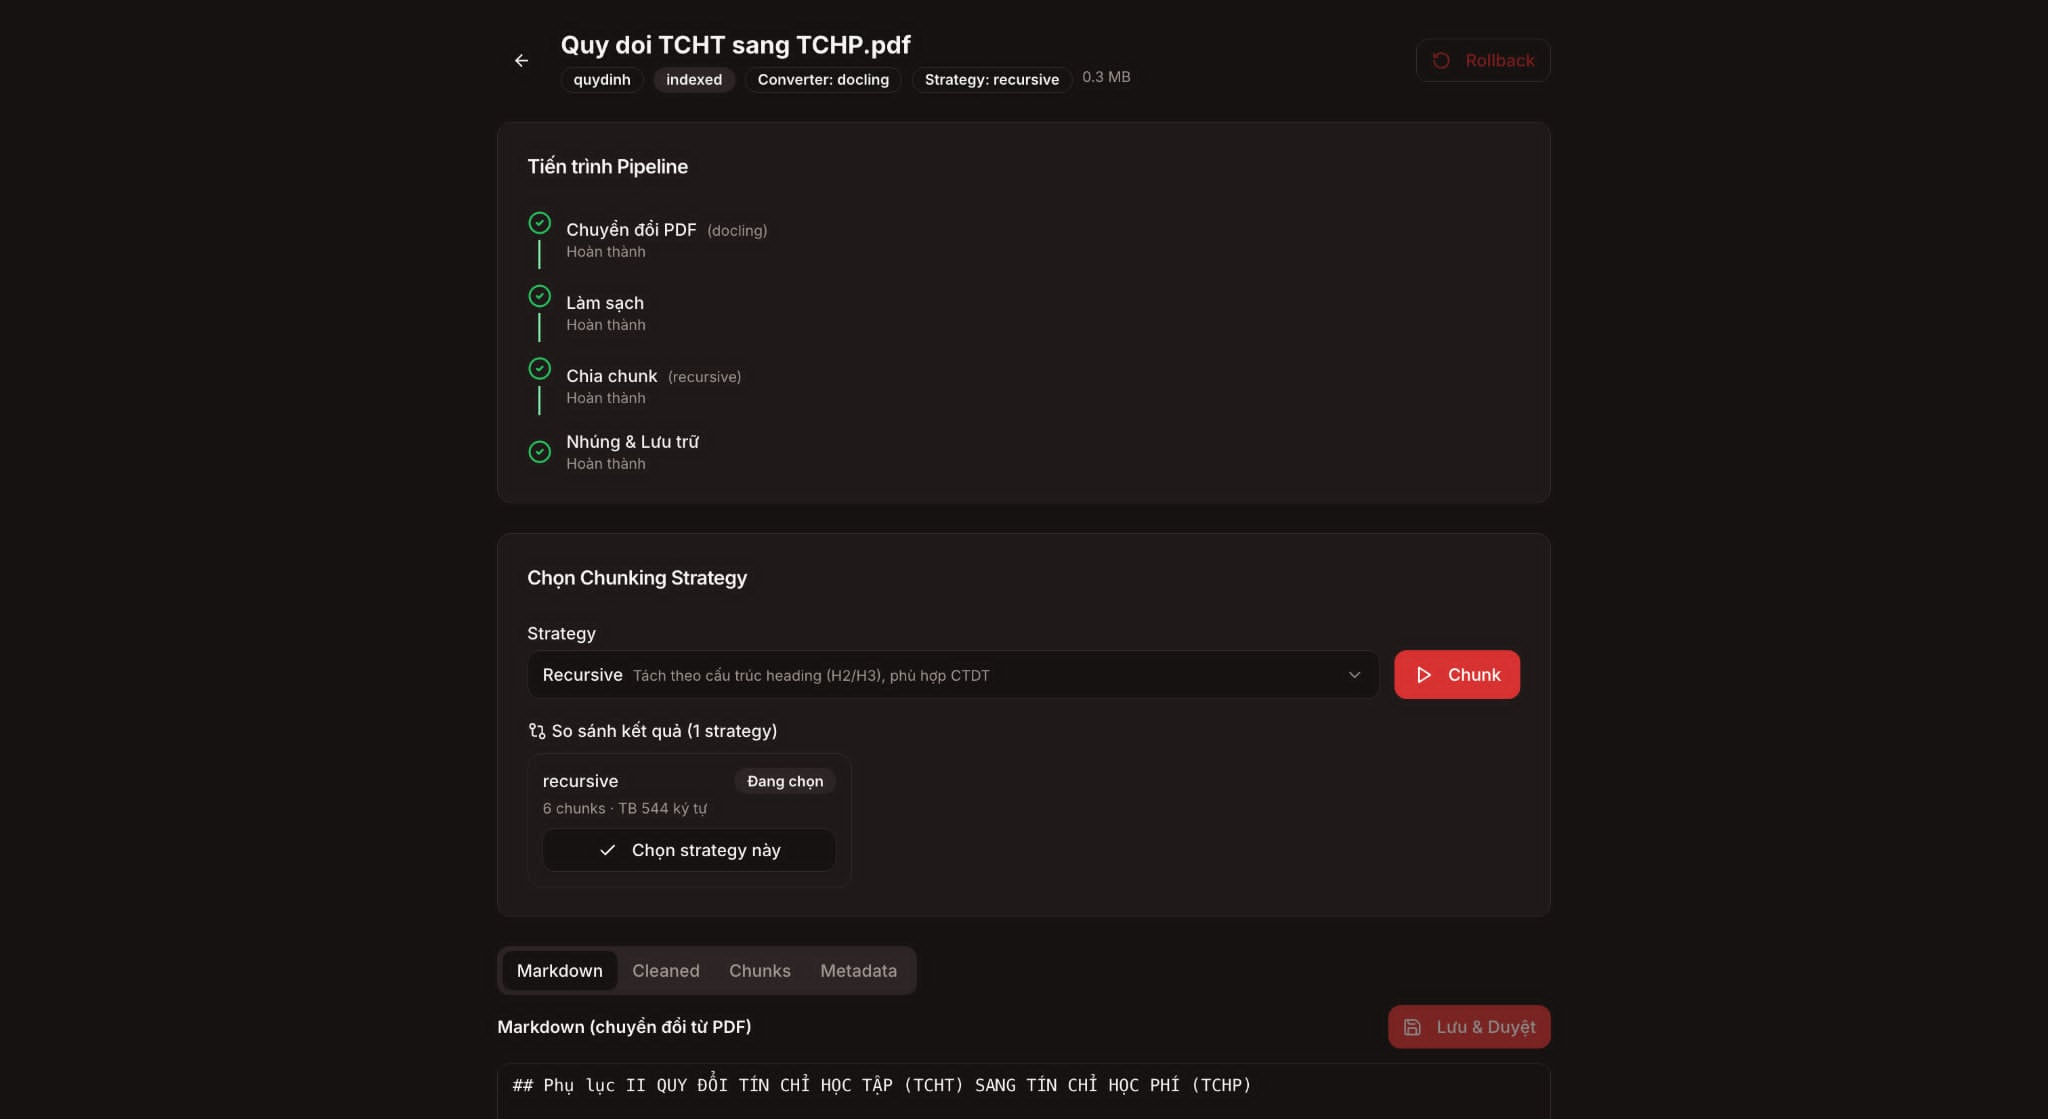
\includegraphics[width=\textwidth,height=2.62cm,keepaspectratio]{figures/ui_admin_review.jpg}
			\end{column}
		\end{columns}
	\end{frame}

	% ================================================================
	\section{Đóng góp nổi bật}

	\begin{frame}{Truy hồi lai cho dữ liệu học vụ}
		\begin{columns}[T,onlytextwidth]
			\begin{column}{0.48\textwidth}
				\begin{block}{Dense retrieval}
					\begin{itemize}
						\item BGE-M3 và E5 multilingual chạy song song.
						\item Phù hợp với câu hỏi diễn đạt khác văn bản gốc.
						\item Tăng độ bao phủ khi một mô hình bỏ sót ứng viên.
					\end{itemize}
				\end{block}
			\end{column}
			\begin{column}{0.48\textwidth}
				\begin{block}{Sparse retrieval}
					\begin{itemize}
						\item BM25 trên Elasticsearch.
						\item Giữ tín hiệu mã môn, mã ngành, khóa, ngày tháng.
						\item Hữu ích với điều khoản và cụm từ chính xác.
					\end{itemize}
				\end{block}
			\end{column}
		\end{columns}

		\vspace{0.35cm}
		\begin{alertblock}{Hợp nhất RRF}
			\small Kết hợp theo thứ hạng giúp ổn định hơn khi cosine similarity và BM25 có thang điểm khác nhau.
		\end{alertblock}
	\end{frame}

	\begin{frame}{Định tuyến theo độ phức tạp}
		\begin{columns}[T,onlytextwidth]
			\begin{column}{0.48\textwidth}
				\begin{block}{Ba nhóm câu hỏi}
					\begin{enumerate}
						\item Chitchat hoặc ngoài phạm vi.
						\item Simple RAG cho câu hỏi rõ nguồn.
						\item Agent cho câu hỏi phức tạp, so sánh, đa nguồn.
					\end{enumerate}
				\end{block}
			\end{column}
			\begin{column}{0.48\textwidth}
				\begin{block}{Ba tầng quyết định}
					\begin{itemize}
						\item Regex xử lý nhanh trường hợp rõ ràng.
						\item Bộ phân loại đa nhãn ước lượng miền tri thức.
						\item LLM chỉ dùng khi câu hỏi mơ hồ hoặc chạm nhiều miền.
					\end{itemize}
				\end{block}
			\end{column}
		\end{columns}
	\end{frame}

	\begin{frame}{Agent Planner--Executor}
		\begin{columns}[T,onlytextwidth]
			\begin{column}{0.48\textwidth}
				\begin{block}{Khi cần agent}
					\begin{itemize}
						\item Câu hỏi so sánh giữa nhiều chương trình.
						\item Câu hỏi cần tổng hợp quy định và kế hoạch.
						\item Câu hỏi nhiều bước hoặc cần đối chiếu logic.
					\end{itemize}
				\end{block}
			\end{column}
			\begin{column}{0.48\textwidth}
				\begin{block}{Cách xử lý}
					\begin{itemize}
						\item Planner chia câu hỏi thành truy vấn con.
						\item Executor truy hồi theo từng miền.
						\item Synthesizer tổng hợp câu trả lời cuối.
						\item Fallback về Simple RAG khi agent lỗi.
					\end{itemize}
				\end{block}
			\end{column}
		\end{columns}
	\end{frame}

	\begin{frame}{Kiểm soát nguồn trước khi trả lời}
		\begin{columns}[T,onlytextwidth]
			\begin{column}{0.48\textwidth}
				\begin{block}{Trước retrieval}
					\begin{itemize}
						\item Chunking theo miền giữ Điều--Khoản, bảng CTĐT, ngày thông báo.
						\item Metadata-aware retrieval lọc theo ngành, khóa, collection và loại tài liệu.
					\end{itemize}
				\end{block}
			\end{column}
			\begin{column}{0.48\textwidth}
				\begin{block}{Sau retrieval}
					\begin{itemize}
						\item ValidityFilter tránh dùng văn bản đã bị thay thế.
						\item ReferenceResolver bổ sung điều khoản được dẫn chiếu.
						\item HyDE fallback khi ngữ cảnh ban đầu yếu.
					\end{itemize}
				\end{block}
			\end{column}
		\end{columns}
	\end{frame}

	\begin{frame}{Tóm tắt đóng góp kỹ thuật}
		\small
		\begin{columns}[T,onlytextwidth]
			\begin{column}{0.48\textwidth}
				\begin{enumerate}
					\item Phân đoạn nội dung theo miền dữ liệu.
					\item Truy hồi lai với BGE-M3, E5 và BM25.
					\item Phân loại độ phức tạp ba tầng.
					\item Phân loại miền với ngưỡng tin cậy.
				\end{enumerate}
			\end{column}
			\begin{column}{0.48\textwidth}
				\begin{enumerate}
					\setcounter{enumi}{4}
					\item Agent Planner--Executor trên LangGraph.
					\item HyDE fallback khi truy hồi yếu.
					\item ValidityFilter và ReferenceResolver.
					\item Admin review trước khi lập chỉ mục.
				\end{enumerate}
			\end{column}
		\end{columns}
	\end{frame}

	% ================================================================
	\section{Kết luận và hướng phát triển}

	\begin{frame}{Kết quả, kiểm thử và triển khai}
		\begin{columns}[T,onlytextwidth]
			\begin{column}{0.47\textwidth}
				\begin{block}{Kết quả nổi bật}
					\scriptsize
					\setlength{\tabcolsep}{3pt}
					\begin{tabular}{|l|c|c|c|}
						\hline
						\textbf{Chỉ số} & \textbf{Vector} & \textbf{BM25} & \textbf{RRF} \\
						\hline
						nDCG@5 & 0,637 & 0,677 & \textbf{0,739} \\
						Recall@5 & 0,660 & 0,733 & \textbf{0,758} \\
						Độ đúng & 75,8\% & 81,2\% & \textbf{83,6\%} \\
						Ảo giác & 3,3\% & 5,4\% & \textbf{2,9\%} \\
						\hline
					\end{tabular}
				\end{block}
			\end{column}
			\begin{column}{0.48\textwidth}
				\begin{block}{Kiểm thử}
					\small
					\begin{itemize}
						\item Routing và reflection.
						\item Retrieval fusion và reranking.
						\item Reference resolution, upload pipeline, cache và agent.
					\end{itemize}
				\end{block}
				\begin{block}{Triển khai}
					\begin{itemize}
						\item FastAPI và web/mobile clients.
						\item MongoDB, Redis, Qdrant, Elasticsearch.
						\item Fallback bật/tắt bằng cấu hình.
					\end{itemize}
				\end{block}
			\end{column}
		\end{columns}
	\end{frame}

	\begin{frame}{Kết luận và hướng phát triển}
		\begin{columns}[T,onlytextwidth]
			\begin{column}{0.48\textwidth}
				\begin{block}{Kết luận chính}
					BKAdvisor là hệ thống RAG học vụ có nhập dữ liệu, truy hồi lai, định tuyến và kiểm soát nguồn.
				\end{block}
				\begin{block}{Thông điệp}
					Câu trả lời học vụ cần đúng nguồn trước khi cần hay; RAG giúp đưa nguyên tắc đó vào pipeline vận hành.
				\end{block}
			\end{column}
			\begin{column}{0.48\textwidth}
				\begin{block}{Hướng phát triển}
					\begin{itemize}
						\item Mở rộng ground-truth đa nguồn.
						\item Đo độ trễ trong môi trường triển khai thật.
						\item Cải thiện metadata và lineage văn bản.
						\item Tối ưu admin review và học từ feedback.
						\item Mở rộng agent cho tác vụ học vụ có cấu trúc.
					\end{itemize}
				\end{block}
			\end{column}
		\end{columns}
	\end{frame}

	\hustthankyou

\end{document}
